%%%%%%%%%%%%%%%%%%%%%%%%%%%%%%%%%%%%%%%%%
% University/School Laboratory Report
% LaTeX Template
% Version 3.1 (25/3/14)
%
%%%%%%%%%%%%%%%%%%%%%%%%%%%%%%%%%%%%%%%%%

%----------------------------------------------------------------------------------------
%   PACKAGES AND DOCUMENT CONFIGURATIONS
%----------------------------------------------------------------------------------------

\documentclass[twocolumn]{article}
\usepackage{graphicx} % Required for the inclusion of images
\usepackage{natbib} % Required to change bibliography style to APA
\usepackage{amsmath} % Required for some math elements

\setlength\parindent{0pt} % Removes all indentation from paragraphs

\renewcommand{\labelenumi}{\alph{enumi}.} % Make numbering in the enumerate environment by letter rather than number (e.g. section 6)

%\usepackage{times} % Uncomment to use the Times New Roman font

%----------------------------------------------------------------------------------------
%   DOCUMENT INFORMATION
%----------------------------------------------------------------------------------------

\title{Experiments in Nuclear Magnetic Resonance} % Title

\author{ } % Author name

\date{\today} % Date for the report

\begin{document}

\maketitle % Insert the title, author and date

\begin{center}
\begin{tabular}{l r}
\end{tabular}
\end{center}

\newcommand{\qel}{electron charge}
\newcommand{\sel}{uncertainty}

% If you wish to include an abstract, uncomment the lines below
\section*{Abstract}

The constituents of matter and their fundamental properties are of great importance to
our understanding and modeling of nature. From consumer technology applications, to weaponry,
astrophysics, and to atmospheric physics, magnetic phenomena dominate many physical reactions
and dictate the interactions of matter and energy we wish to predict. Here, I measured the
intrinsic dipole moment of the proton with a glycerine probe and used the results to characterize an electromagnet,
and attempted to find the magnetic dipole moment of an atomic nucleus. The measured value
on the proton was $7.903 \times 10^{-11}$ eV/G $\pm 1.0 \times 10^{-12}$ eV/G. The results
of the magnet modeling were that the B field increases linearly with voltage (or current), and the data
and results will be discussed in further detail in later sections. Given the magnetic field strength
and resonant frequency, the unknown probe appears to be Fluorine.


\section*{Introduction}

The energy of a dipole in a magnetic field is simply the inner product of the dipole moment
and the magnetic field strength. A dipole 'flipping' from being antiparallel with the field to being
parallel is then
\begin{equation}
\Delta E = 2 \mu B
\end{equation}
A photon or electromagnetic wave released by this would then have the energy
\begin{equation}
f = \frac{2 \mu B}{h}
\end{equation}
After the nuclear dipole moments align with the external field, this energy is no longer
being released. Boltzmann statistics show this happens on time scales much shorter than a second,
so a set of Helmholtz coils, being driving by a $120$ Hz AC current serve to scramble the
dipole alignment.
The probe holding the sample includes a marginal oscillating antenna, which provided the
electromagnetic radiation to perturb the dipoles.
Finally, because the energy released is dependent on the magnetic field strength and direction,
it is then important to ensure a uniform field over the volume of the sample. This was done
by having the samples be on the end of a long probe that sits directly in the center of
two flat magnet faces.

\section*{Procedure}

The initial measurement was that of the proton magnetic moment in a fixed permanent magnet. I used a
Hall Effect teslameter to find the magnetic field of the permanent magnet. Several measurements show $540$ mT, and
the characteristic resonant frequency for the glycerine sample for this magnetic field strength was $20.627$ MHz. This was done by connecting
the signal from the antenna to an oscillocope. The frequency of the marginal ocillator is controlled
by a fine tuning knob on the probe. When the frequency was resonant with the proton, the signal on the oscilloscope
shows peaks seperated in time, which can be tuned until they are equally spaced in time. Then, a Radio Shack radio was
used to find this frequency.

Given the emperical number for the magnetic moment, I began to characterize the electromagnet. I set the
radio to 16.0Mhz, tuned the marginal oscillating antenna to this frequency, then found the matching current
that would induce resonance. The radio and antenna would be tuned up $0.5$ Mhz, and the process would continue.

Finally, finding the magnetic resonance of the unknown sample was done in kind using the electromagnet. I set the
radio to $19.000$ MHz, tuned the marginal oscillating antenna to roughly that frequency, then scanned over the possible
currents from the electromagnet until finding resonance. Then, each parameter was tuned to find resonance.

\section*{Analysis}

The proton magnetic moment was found using equation $2$, and all reported uncertainties were calculated
using strategies outlined in Chapter 3 of {\it An Introduction to Error Analysis} by John Taylor.

To find the relationship between magnetic field strength and current of the electromagnet, I used the polyfit package from the
python library numpy. The slope of the fit is $124.5$, with an intercept of $2.4$, although naturally, with no current,
the electromagnet has no magnetic field.

I found the magnetic moment of the unknown probe using the same method outlined for the glycerine sample,
and converted it into units of $5.05505 \times 10^{24}$ erg/gauss {\it CRC Handbook of Chemistry and Physics, 49th Edition}.
This number most closely matched that of Fluorine.

\begin{figure}
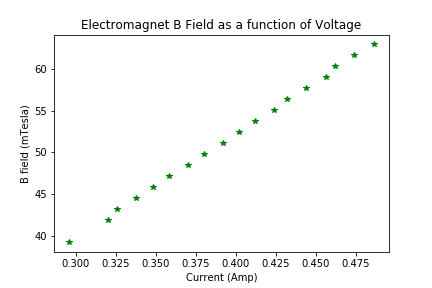
\includegraphics[width=\linewidth]{nmr_fig_1.png}
\caption{Graph of B field vs. current}
\label{fig:graph1}
\end{figure}
  \section*{Conclusion and Remarks}

I feel my measurement of the proton magnetic moment accurately reflects numbers reported elsewhere, and found this to be
an accurate way of making this measurement. The characterization of the electromagnet is very subjective to the intial dipole
measurement, but it was used (presumeably) correctly to characterize the unknown probe. Various bits of uncertainty found their ways
all the way through the problem, including relying on the Hall Effect sensor to reliably measure the B field of the permanent magnet.
The reading of this meter was very dependent of position and angle relative to the magnet, making getting a truly 'accurate' reading of
the magnet difficult. The results all depend on this reading, and so increasing the accuracy would improve the accuracy of the results.

However, given the linearity of the B field vs. Current graph, as long as strong enough B fields can be made, this method could be used
to identify many substances. It raises other questions, including magnetic moments of other subatomic particles, and the implications
of those values.

\section*{Appendix}
\subsection*{References}
Wolfram Alpha; http://www.wolframalpha.com

Python, numpy; http://www.python.org

CRC Handbook of Chemistry and Physics 49th Ed.

An Introduction to Error Analysis; Taylor, John R.

\newpage
\subsection*{Data}
\begin{table}[h!]
  \begin{center}
    \label{tab:table1}
    \caption{Data as recorded while characterizing electromagnet}
    \begin{tabular}{l c r}
      \textbf{Voltage (mV)} & \textbf{Frequency (MHz)}\\
      \hline
      14.8 & 15.0000\\
      16.0 & 16.002\\
      16.3 & 16.501\\
      16.9 & 17.005\\
      17.4 & 17.502\\
      17.9 & 18.001\\
      18.5 & 18.500\\
      19.0 & 19.000\\
      19.6 & 19.500\\
      20.1 & 19.998\\
      20.6 & 20.500\\
      21.2 & 21.000\\
      21.6 & 21.501\\
      22.2 & 22.000\\
      22.8 & 22.501\\
      23.1 & 23.000\\
      23.7 & 23.500\\
      24.3 & 24.000
    \end{tabular}
  \end{center}
\end{table}
\end{document}
~
